%
% File acl2020.tex
%
%% Based on the style files for ACL 2020, which were
%% Based on the style files for ACL 2018, NAACL 2018/19, which were
%% Based on the style files for ACL-2015, with some improvements
%%  taken from the NAACL-2016 style
%% Based on the style files for ACL-2014, which were, in turn,
%% based on ACL-2013, ACL-2012, ACL-2011, ACL-2010, ACL-IJCNLP-2009,
%% EACL-2009, IJCNLP-2008...
%% Based on the style files for EACL 2006 by 
%%e.agirre@ehu.es or Sergi.Balari@uab.es
%% and that of ACL 08 by Joakim Nivre and Noah Smith

\documentclass[11pt,a4paper]{article}
\usepackage[hyperref]{acl2020}
\usepackage{times}
\usepackage{placeins}
\usepackage{latexsym}
\usepackage{graphicx}
\usepackage[skip=10pt plus1pt, indent=20pt]{parskip}
\usepackage{url}
\renewcommand{\UrlFont}{\ttfamily\small}

% This is not strictly necessary, and may be commented out,
% but it will improve the layout of the manuscript,
% and will typically save some space.
\usepackage{microtype}

\aclfinalcopy % Uncomment this line for the final submission
%\def\aclpaperid{***} %  Enter the acl Paper ID here

%\setlength\titlebox{5cm}
% You can expand the titlebox if you need extra space
% to show all the authors. Please do not make the titlebox
% smaller than 5cm (the original size); we will check this
% in the camera-ready version and ask you to change it back.

\newcommand\BibTeX{B\textsc{ib}\TeX}

\title{The Dark Side of Language: Using NLP to Combat Hate Speech}

\author{ 
  Shalini Chawla, shalini\_chawla@berkeley.edu
  \\[2ex]
  \textbf{Adam Hyman, adamhyman@berkeley.edu}
  \\[2ex]
  \textbf{Sreeram Ravinoothala, sreeram@berkeley.edu} 
  }

\date{April 2023}

\begin{document}
\maketitle
\begin{abstract}
With the advent of social media, people have had access to propagate hate anonymously, making it more dangerous than ever as the impact is not contained by a social group or geographic area any more. It is very important for social media companies to accurately identify hateful content and a lot of work has been already done to classify online content as toxic vs non-toxic for content moderation. We would like to extend this classification from binary to a a multi label classification and identify the specific hate categories toxic content belongs to. This information can be used by socio-political studies exploring the relationship between specific social-political events and their impact on triggering hateful content in online media. In this paper, we fine-tune three pre-trained large language models for a multi-label classification task to categorize text comments as toxic, severe\_toxic, obscene, threat, insult and identity\_hate. To tackle the imbalance of available training data, we use back translation using multiple intermediate to augment training data for the minority classes.

\end{abstract}

\section{Introduction}

Social media brings people from all areas of society to shared spaces.  While a wide-variety of view points is usually a good thing, there is a small minority of speech, hate speech, that social media platforms consider to be hurtful to the platform and the community they're trying to build.  Hate speech can be targeted against and individual or group based on inherent characteristics, like race or gender.  The offensive speech disrupts social peace on these platforms and upsets the users.  The social media platforms use considerable resources to remove hate speech, by allowing users to flag offensive content and with automated algorithms, so the negative effects can be mitigated as soon as possible.

With the advances in machine learning, many of the social media platforms have done a lot of great work in controlling the proliferation of hate speech by making use of classification algorithms but there is much more to be done to reduce the exposure to a great extent. They are successful in many ways but classifying the content to check if it indeed is hate is very complex as it depends on the context as well as whether its used loosely. There is lot of research done or going on classifying the text as well as augmenting such text.

The ability in building accurate models to correctly classify hateful content is a challenging task due to the limited availability of labeled data required for training. The training data needs to be labeled by human annotators. In addition to being a tedious task, it also exposes the annotators to the disturbing content in the data they are required to label. The public data sets available today are highly imbalanced and have very limited samples for some of the minority categories including threat, obscene and severe\_toxic compared to the large amount of non-toxic samples. We follow two approaches to deal with the limitations of data availability.

1) Pre-trained large language models have made it feasible to achieve better accuracy  in many NLP tasks where the amount of training data is limited, by providing word embeddings that have already learned characteristics of natural language. Using these pre-learned embeddings as the input to a classification model enables the model to learn to classify the content using much lesser amount of training data than it would have needed to learn the same relationship from scratch.

We use three large language models: BERT, T5 and XLNet and fine-tune them for a multi label classification task using our data set that has been labeled with the 6 toxicity classes. 

2) Our source data set is highly imbalanced and has very limited data for three out of the six categories. We use a combination of approaches to balance our data set to help the model balance learning across all categories. 
We have three minority categories: threat, severe-toxic and identity\_hate that have very low representation in our training data set. We use the TOXIGEN \cite{hartvigsen2022toxigen} data set to augment data for the identity\_hate class. To augment data for the other classes, we use back translation to generate additional samples from the existing data. 


\section{Background}
There has been a lot of research and previous work done with focus on toxic content  classification and a few different pathways have been explored to improve the accuracy of classification. 
The unavailability of enough quality labeled data has been widely accepted as a limitation in the ability to create accurate models for toxic content classification. \cite{rastogi2020can} has explored generating synthetic data using EDA and back translation to augment the training data and reported improved recall and F1 scores. \cite{hartvigsen2022toxigen} have explored the complexity of identifying implicit identity\_hate targeted at minority groups and used GPT-2 to generate additional data to augment the current available human labeled data sets. 
Another issue has been the inconsistency in labeling across the publicly available data sets limiting the generalization of trained models. 

\section{Data}

\subsection{Source Data Set}
We used the dataset from the Jigsaw Toxic Comment Classification Challenge held by Kaggle, that contains Wikipedia comments, that were labelled by human raters for various types of toxic content.  The data set consist of 3 files that includes the labeled training data, test data and the test labels (that was made available after the competition concluded).  We combine the test data and labels file by joining them on the unique comment identifiers. The training data set has 160,000 comments while the test data set has 64,000 comments. We converted the comments into lowercase and cleaned the contents by removing punctuation and special characters. Once processed both the training and test data  consisted of the text comments and binary labels for the 6 categories:

\begin{itemize}
\item toxic
\item severe\_toxic
\item obscene
\item threat
\item insult
\item identity\_hate
\end{itemize}



\subsection{Data Balancing}
Our source data is highly imbalanced. Out of the 6 labeled classes, 3 are majority classes with and 3 are minority classes.


\begin{figure}[h!]
\centering
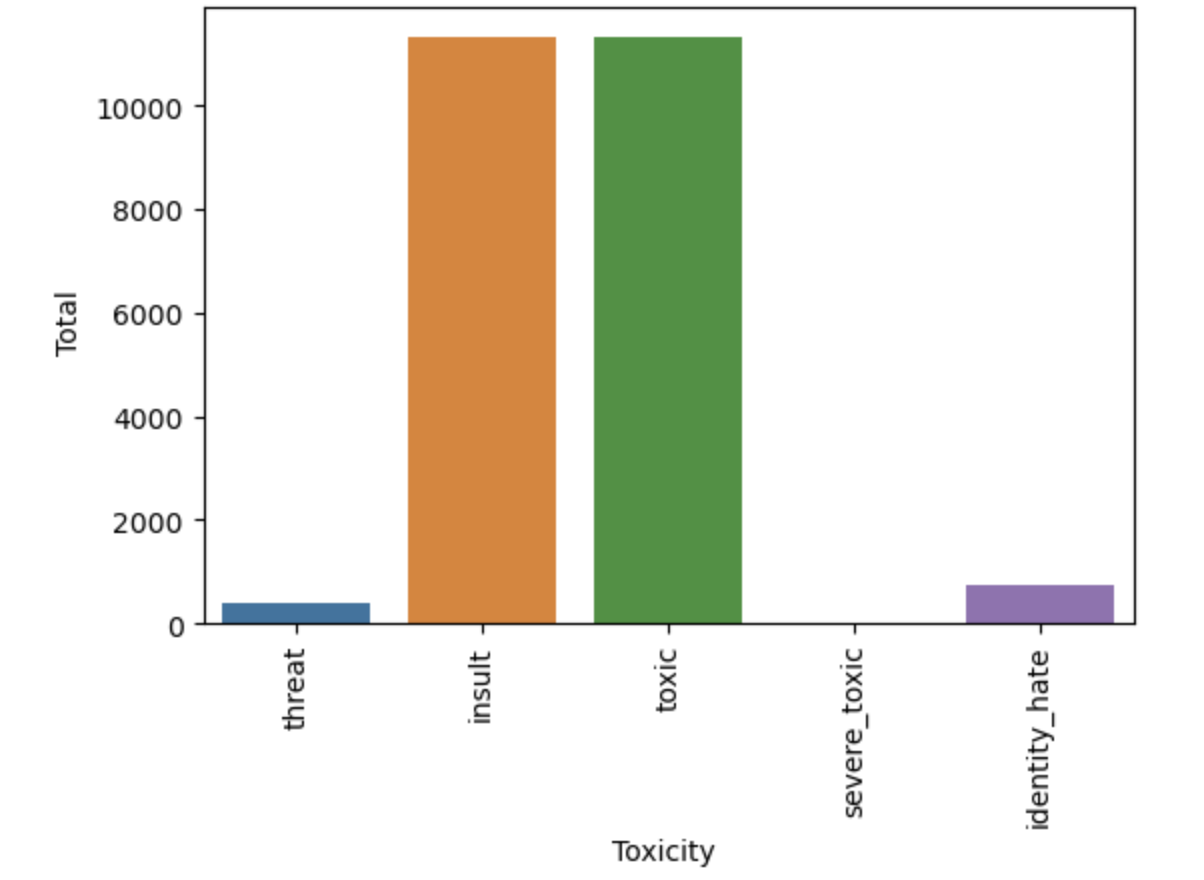
\includegraphics[width=50mm,scale=0.5]{label_counts.png}
\caption{Toxicity Label Count}
\label{Fig1. label count vs toxicity}
\end{figure}


\subsection{Augmenting Minority Class Data}
We augmented the training data for minority classes to bring it closer in count to the majority classes.

For \emph{severe\_toxic} and \emph{threat}, we used back-translation with Google Translate API to supplement the training data.  For the smallest class, \emph{threat}, we back-translated all 476 comments using 3 languages - Chinese, Hindi and French - which along with the original comment quadrupled the number of comments in our training data.  For \emph{severe\_toxic}, we back translated 500 comments using Chinese, to supplement our training data.

We supplemented \emph{identity\_hate} with 640 records created by Microsoft's Toxigen repository, which uses a large scale pre-trained language model and a classifier to generate synthetic hate speech.  The repository includes two methods for generating hate speech:  Demonstration-Based Prompting and an adversarial set up between a classifier and a generator.  We included 320 records from each of the methods.

\subsection{Undersampling Majority Class Data}
To further balance the data set for the 6 identified classes, we selected all comments labelled with the minority classes, including augmented data.  Since many of these comments are also labelled with the majority classes, we only needed to select a small amount of additional comments, that were labelled with the majority classes, but not the minority classes, in order to get a data set that was approximately balanced.


\begin{figure}[h!]
\centering
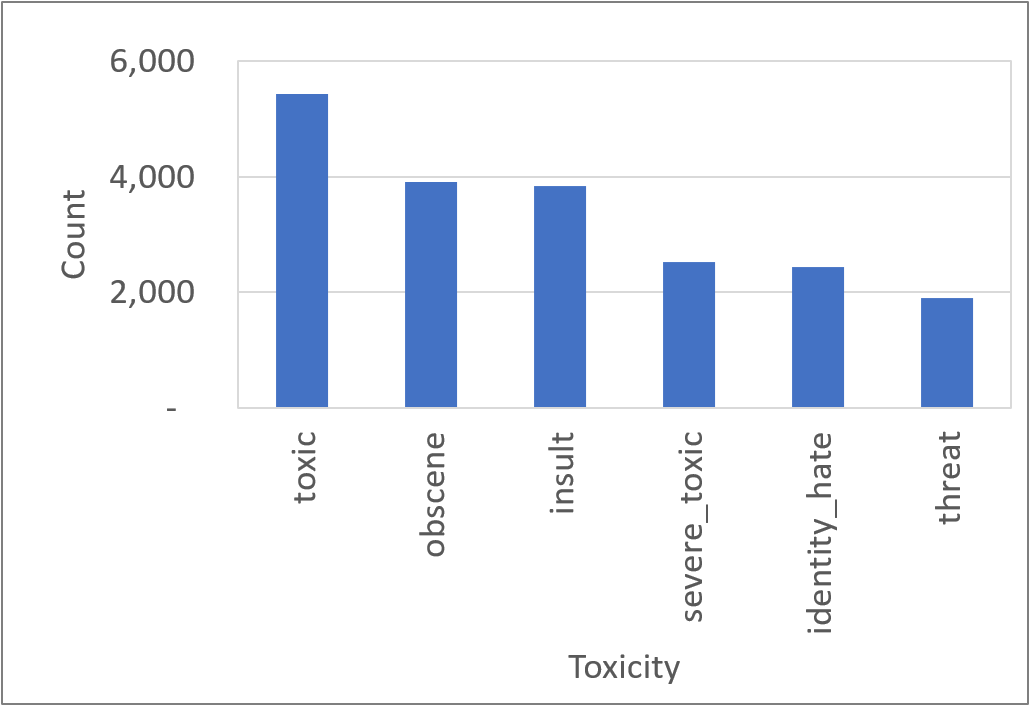
\includegraphics[width=50mm,scale=0.5]{label_counts_balanced.png}
\caption{Label Count for Balanced Data}
\label{Fig2. label count vs toxicity}
\end{figure}


\section{Methods}

\subsection{Baseline Model - BERT fine-tuned on source data}
Our baseline model is BERT base model(cased). We fine-tune the model on the full training data set that has been split into training and validation using 80:20 split and stratified on the 6 label classes. We add a hidden layer with 200 neurons and dropout layer with 0.3 before our final classification layer with 6 outputs to perform a multi label classification. We train the model for 2 epochs using learning rate of .00005 and batch size of 32.

The model performs really poorly for our 3 minority classes, completely failing to identify any of the severe\_toxic, threat and identity\_hate comments.

\begin{table}
\centering
\begin{tabular}{lrrr}
\hline
\textbf{class} & \textbf{prec} & \textbf{recall} & \textbf{f1-score}\\
\hline
\verb|toxic| & 0.62 & 0.40 & 0.49 \\
\verb|severe_toxic| & \textcolor{red}{0.00} & \textcolor{red}{0.00} & \textcolor{red}{0.00} \\
\verb|obscene| & 0.66 & 0.32 & 0.43 \\
\verb|threat| & \textcolor{red}{0.00} & \textcolor{red}{0.00} & \textcolor{red}{0.00} \\
\verb|insult| & 0.65 & 0.25 & 0.36 \\
\verb|identity_hate| & \textcolor{red}{0.00} & \textcolor{red}{0.00} & \textcolor{red}{0.00} \\
\vspace{2\baselineskip}\\
\verb|micro avg| & 0.64 & 0.31 & 0.42 \\
\verb|macro avg| & 0.32 & 0.16 & 0.21 \\
\verb|weighted avf| & 0.58 & 0.31 & 0.40 \\
\verb|samples avg| & 0.04 & 0.03 & 0.03 \\
\hline
\end{tabular}
\caption{Baseline Model - Classification Report}
\end{table}

\subsection{BERT fine-tuned with balanced data}
Our baseline model's poor performance is due to the much smaller amount of training data for the minority classes. To model is favoring the majority classes and is learning to just return the label as one of the majority classes to maximize accuracy since that is what most of the data is. To help our model learn the features of the minority classes, we create a new balanced data set by undersampling our majority classes and augmenting the minority classes. We run the BERT model with the same hyperparameters as in our baseline with the balanced data set.
Balancing the data set did not improve the classification score for minority classes at all it still stayed flat at 0 with none of the 3 minority classes being identified. Our data set size was reduced drastically after undersampling but we still had ~13,000 records which is an acceptable amount of data for fine-tuning BERT.
Since BERT was originally trained on wikipedia data and has not previously seen a majority of the vocabulary that is in the toxic data, it is not able to learn enough from the provided data to identify the minority classes. 


\subsection{Retraining BERT layers}
Our next step was to systematically unfreeze the pre-trained BERT layers 2 at a time and retrain them using our data set. We used the original unbalanced data set and the balanced dataset we created and re-trained the top 2 BERT layers, followed by 4, 6 and all the layers.
The first classifier with retraining only the top 2 BERT layers gave as a huge improvement in score for all three of the minority classes. As we retrained deeper layers, the total score kept moving upwards. For the full unbalanced dataset, the improvement stagnates after 4 layers. This has been observed in previous work done by \cite{Singh2020HowMD}. But we observed that with the smaller balanced dataset, the improvement continues as we retrain more layers with full retraining of all 12 layers giving us the best scores.


\subsection{T5}
We used T5-small \cite{raffel2020exploring} on the unbalanced training dataset similar to BERT. The model was adopted from \cite{t5mlcode}. As part of the multilabel classification a language modeling head is used on top of the decoder. The model was run 2 epochs with 8 and 16 batch size. The lesser epochs was because of the time the model was taking to train and predict. The model was very biased towards the higher dataset and also failed to predict the lower classes (insult, identity\_hate) which can be seen from the lower ROC-AUC scores.

The same experiment was repeated with balanced dataset for 2 epochs and 16 batch size. The results were similar to what was seen with unbalanced dataset. It was still not predicting the classes insult and identity\_hate properly.

With above results, it was not prudent for us to pursue with T5 due to no improvement in the metrics.

\subsection{XLNet}

Once T5 didn't give an improvement over Bert, we examined models that use a different approach to pre-training and implemented XLNet (\cite{yang2019xlnet}, which is an auto-regressive based model that does a better job of learning dependency pairs.

We ran XLNet on both the unbalanced and balanced data, for 6 epochs on each.

We found that XLNet gave us a modest improvement over Bert, both with balanced and unbalanced data.

\FloatBarrier
\section{Results and Discussion}

\begin{table*}

\centering
\begin{tabular}{lrrrrrrrrrr}
\hline
\textbf{Model} & \textbf{Macro} & \textbf{Macro} & \textbf{Toxic} & \textbf{Severe Toxic} & \textbf{Obscene} & \textbf{Threat} & \textbf{Insult} & \textbf{Id Hate}
\\
\textbf{ } & \textbf{F1} & \textbf{AUC} & \textbf{AUC} & \textbf{AUC} & \textbf{AUC} & \textbf{AUC} & \textbf{AUC} & \textbf{AUC}\\
\hline
\verb|BERT Baseline|&0.20 & 0.56 & 0.66 & 0.50 & 0.63 & 0.50 & 0.61 & 0.50 \\
\verb|BERT 2-layers| & 0.50 & 0.74 & 0.88 & 0.60 & 0.87 & 0.57 & 0.80 & 0.71 \\
\verb|BERT 4-layers| & 0.55 & 0.78 & 0.90 & 0.59 & 0.86 & 0.71 & 0.88 & 0.72 \\
\verb|BERT 6-layers| & 0.58 & 0.85 & 0.91 & 0.83 & 0.89 & 0.85 & 0.87 & 0.73 \\
\verb|BERT 12-layers| & 0.49 & 0.77 & 0.90 & 0.73 & 0.89 & 0.49 & 0.88 & 0.73 \\
\verb|T5| & 0.07 & 0.59 & 0.53 & 0.94 & 0.51 & 0.58 & 0.50 & 0.50 \\
\verb|XLNet| & 0.60 & 0.82 & 0.90 & 0.69 & 0.87 & 0.75 & 0.87 & 0.85 \\
\hline
\end{tabular}
\caption{Metrics - All Models trained with original unbalanced data}
\label{table:UnBalResults}
\end{table*}

\begin{table*}
\centering
\begin{tabular}{lrrrrrrrrrr}
\hline
\textbf{Model} & \textbf{Macro} & \textbf{Macro} & \textbf{Toxic} & \textbf{Severe Toxic} & \textbf{Obscene} & \textbf{Threat} & \textbf{Insult} & \textbf{Id Hate}
\\
\textbf{ } & \textbf{F1} & \textbf{AUC} & \textbf{AUC} & \textbf{AUC} & \textbf{AUC} & \textbf{AUC} & \textbf{AUC} & \textbf{AUC}\\
\hline
\verb|Bert Baseline| & 0.05 & 0.51 & 0.57 & 0.5 & 0.50 & 0.49 & 0.50 & 0.50 \\
\verb|Bert 2 layers| & 0.42 & 0.86 & 0.85 & 0.79 & 0.87 & 0.91 & 0.83 & 0.89 \\
\verb|Bert 4 layers| & 0.44 & 0.87 & 0.60 & 0.88 & 0.87 & 0.92 & 0.83 & 0.88 \\
\verb|Bert 6 layers| & 0.50 & 0.83 & 0.87 & 0.73 & 0.83 & 0.88 & 0.79 & 0.90 \\
\verb|Bert 12 layers| & 0.51 & 0.89 & 0.89 & 0.87 & 0.88 & 0.90 & 0.87 & 0.91 \\
\verb|T5| & 0.12 & 0.61 & 0.77 & 0.92 & 0.52 & 0.49 & 0.50 & 0.50 \\
\verb|XLNet| & 0.42 & 0.90 & 0.89 & 0.83 & 0.90 & 0.95 & 0.89 & 0.93 \\
\hline
\end{tabular}
\caption{Metrics - All Models trained with augmented balanced data}
\label{table:BalResults}
\end{table*}

Metrics were captured across multiple models that were tested as shown in Table ~\ref{table:UnBalResults} and Table ~\ref{table:BalResults}. Each model was run for multiple epochs to ensure proper outcome of metrics. We captured macro AUC-ROC scores, macro F1 score and AUC-ROC scores for different labels across different runs.

The baseline BERT model (with no re training) performed very poorly on the minority classes for both Unbalanced and Augmented Balanced dataset. We fine tuned the model by unfreezing multiple layers and training BERT to learn the toxic data. As can be seen in the tables, there was a significant improvement in the F1, AUC-ROC scores. We also saw the minority classes performing well in this situation.

T5 was applied on unbalanced data and balanced data. The observations showed that T5 does worse on all of our metrics compared to BERT and XLNet with the exception of classifying severe\_toxic data where it outperforms all the other runs with huge margin.

Similarly XLNet model was applied on both unbalanced as well as balanced dataset. We observed that XLNet outperformed all of our runs with other models for both the datasets. 

Overall, the metrics across all the labels are more uniformly distribured when the models are trained on the balanced dataset. Referring to Figures ~\ref{UnbalancedData} and ~\ref{BalancedData} there is a clear indication of how each model shines given a balanced dataset.

\begin{figure}[]
\centering
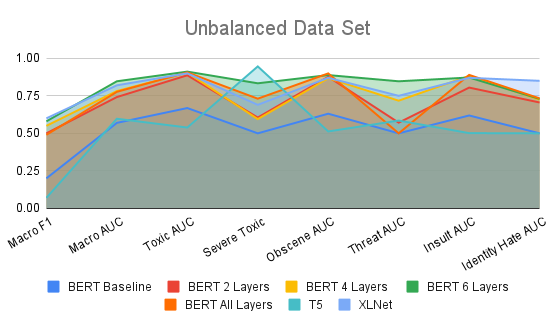
\includegraphics[width=75mm,scale=0.5]{Unbalanced Data Set.png}
\caption{Unbalanced Data set}
\label{UnbalancedData}
\end{figure}

\begin{figure}[]
\centering
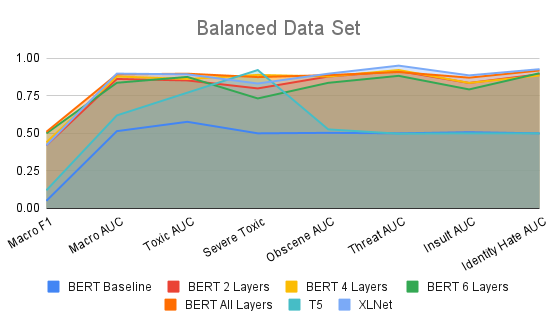
\includegraphics[width=75mm,scale=0.5]{Balanced Data Set.png}
\caption{Balanced Data set}
\label{BalancedData}
\end{figure}
\FloatBarrier

\section{Conclusion}
In conclusion we found that the benefits of a pre-trained large language model are limited by the vocabulary that it was trained on. With Bert being trained only on wikipedia data it hasn't seen the same level of toxic content as in our training dataset which makes it harder to classify toxic comments correctly.
T5 was pre-trained on a big corpus of data (C4) where it would have picked up some toxic labels. The metrics for severe\_toxic in Table ~\ref{table:BalResults} as well as ~\ref{table:UnBalResults} clearly shows that it is biased towards that label due to some pre-learning whereas few other classes were left out.
With XLNet outshining the other two models in the metrics, we can clearly say that XLNet can be used for multi label classification on toxic data

\section{Future work}
Our experiments with different models were based on the toxic dataset and some augmentation that was done to balance it. One area we did not focus on is unbiased training or providing unbiased dataset. So, there may be some biases that are exhibited with the training we did for the dataset we obtained. This is one area we can look at in the future.

For future work we would like to evaluate and optimize our model for fairness across sensitive groups inspired by \cite{baldini2021your}.

We have seen that each of the model has its own area of strength. So, we would like to create and  ensemble model derived from the strengths shown by BERT, T5 and XLNet. 

\bibliographystyle{apalike}
\bibliography{acl2020}
\end{document}
